\documentclass{beamer}
\usetheme{Madrid}
\usecolortheme{default}
\usepackage{listings}
\usepackage{tcolorbox}
\tcbuselibrary{listings, skins}

\newtcblisting{mycode}{
  arc=0mm,                          % Sharp corners
  boxrule=0.5pt,                    % Border thickness
  colback=white,                    % Background color
  colframe=black,                   % Border color
  listing only, 
  listing options={
    language=Python,
    basicstyle=\small\ttfamily,      % Monospace font
    keywordstyle=\color{blue},       % Color for 'import', etc.
    commentstyle=\color{blue},       % Color for comments
    stringstyle=\color{red},
    showstringspaces=false,
    breaklines=true
  },
  sharp corners,
  enhanced,
}
\usepackage{listings}
\usepackage{graphicx}

\lstset{
    language=Python,
    basicstyle=\ttfamily\small,
    keywordstyle=\bfseries,
    showstringspaces=false,
    breaklines=true
}

\title{Probability-3.0.44}
\author{SAI HASINI PAPPULA-EE25BTECH11044}
\date{\today}

\begin{document}
\begin{frame}
\titlepage
\end{frame}
\begin{frame}{Question}
Let $X$ be a random variable following normal distribution with mean $+1$ and variance $4$. 

Let $Y$ be another normal variable with mean $-1$ and variance unknown. If
\[
P(X \le -1) = P(Y \ge 2),
\]
the standard deviation of $Y$ is:

\begin{itemize}
    \item[(a)] 3
    \item[(b)] 2
    \item[(c)] $\sqrt{2}$
    \item[(d)] 1
\end{itemize}
\end{frame}

%------------------------------------------------

\begin{frame}{Standardization (Z-Transformation)}
\textbf{Idea:} Convert any normal random variable into a \textit{standard normal variable}.

\begin{itemize}
    \item If $X \sim N(\mu, \sigma^2)$, we define:
\end{itemize}

\[
Z = \frac{X - \mu}{\sigma}
\]

\begin{itemize}
    \item This transformation shifts the mean to $0$ and scales the variance to $1$
    \item So, $Z \sim N(0,1)$ (standard normal distribution)
    \item This allows us to use standard normal tables for probability calculation
\end{itemize}

\end{frame}

%------------------------------------------------

\begin{frame}{Step 1: Standardize $X$,$Y$}
Given: $X \sim N(1,4)$, so $\sigma = 2$

\[
P(X \le -1) = P\left(Z \le \frac{-1 - 1}{2}\right)
\]
\[
= P(Z \le -1)
\]

Given: $Y \sim N(-1,\sigma^2)$

\[
P(Y \ge 2) = P\left(Z \ge \frac{2 - (-1)}{\sigma}\right)
\]
\[
= P\left(Z \ge \frac{3}{\sigma}\right)
\]
\end{frame}

%------------------------------------------------

\begin{frame}{Step 2: Equate Probabilities}
\[
P(Z \le -1) = P\left(Z \ge \frac{3}{\sigma}\right)
\]

Using symmetry of normal distribution:
\[
P(Z \le -1) = P(Z \ge 1)
\]

So,
\[
P(Z \ge 1) = P\left(Z \ge \frac{3}{\sigma}\right)
\]

\end{frame}

\begin{frame}{Final Answer}
\[
\frac{3}{\sigma} = 1
\]
\[
\sigma = 3
\]
\begin{block}{Conclusion}
\textbf{Option (a): $\sigma = 3$ is correct.}
\end{block}
\end{frame}

\begin{frame}[fragile]
\frametitle{Python Code for Plot}

\begin{mycode}
import numpy as np
import matplotlib.pyplot as plt
from scipy.stats import norm
 
# Parameters
mu_X, sigma_X = 1, 2      # X ~ N(1, 4)
mu_Y, sigma_Y = -1, 3     # Y ~ N(-1, 9)
 
# Range for plotting
x = np.linspace(-10, 10, 1000)
 
# PDFs
pdf_X = norm.pdf(x, mu_X, sigma_X)
pdf_Y = norm.pdf(x, mu_Y, sigma_Y)
\end{mycode}

\end{frame}
\begin{frame}[fragile]
\frametitle{Python Code for Plot}

\begin{mycode}

# Plot curves
plt.figure(figsize=(8, 4))
plt.plot(x, pdf_X, linewidth=1.8,
         label=r'$X \sim \mathcal{N}(1,\,4)$')
plt.plot(x, pdf_Y, linewidth=1.8,
         label=r'$Y \sim \mathcal{N}(-1,\,9)$')
        
 # Shade P(X <= -1)
x_fill_X = np.linspace(-10, -1, 500)
plt.fill_between(x_fill_X,
                 norm.pdf(x_fill_X, mu_X, sigma_X), alpha=0.3, label=r'$P(X \leq -1)$')

\end{mycode}

\end{frame}

\begin{frame}[fragile]
\frametitle{Python Code for Plot}

\begin{mycode}
# Shade P(Y >= 2)
x_fill_Y = np.linspace(2, 10, 500)
plt.fill_between(x_fill_Y,
               norm.pdf(x_fill_Y, mu_Y, sigma_Y),
               alpha=0.3, label=r'$P(Y \geq 2)$')
 
# Labels and formatting
plt.title(r'$P(X \leq -1)$ and $P(Y \geq 2)$', fontsize=12)
plt.xlabel('x'); plt.ylabel('Probability Density')
plt.legend(fontsize=10)
plt.grid(True, linestyle='--', alpha=0.5)
plt.tight_layout()
plt.savefig('plot4.png', dpi=150)

\end{mycode}

\end{frame}

\begin{frame}{Graph of the Solution}
\begin{center}
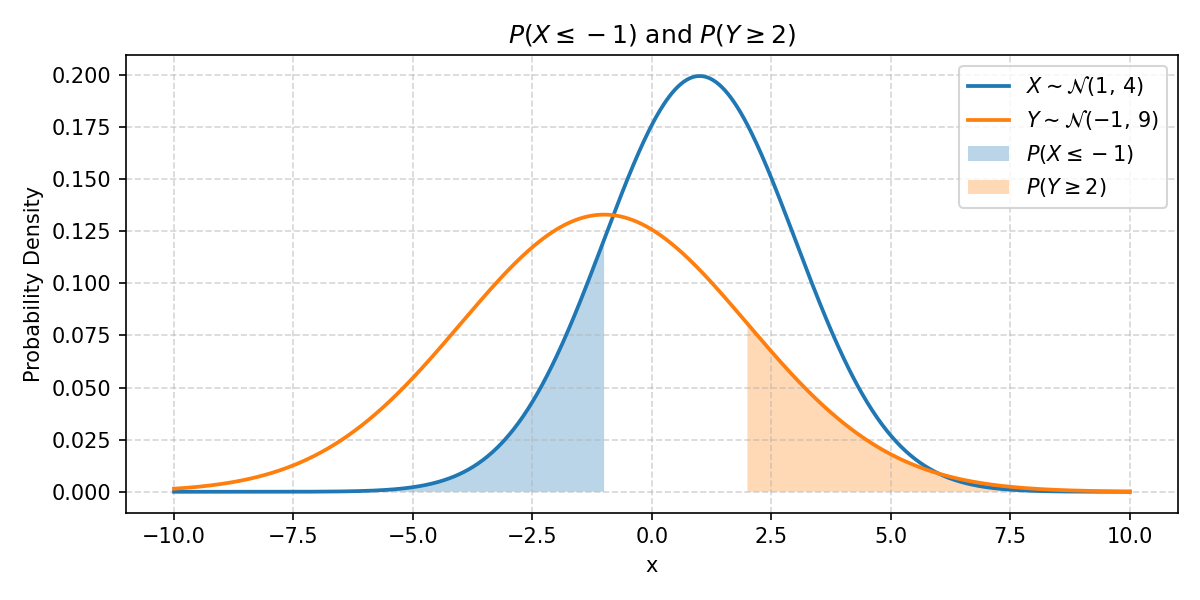
\includegraphics[width=0.8\textwidth]{plot4.png}
\end{center}
\begin{itemize}
  \item Shaded left tail: $P(X \leq -1)$ where $X \sim \mathcal{N}(1,\,4)$
  \item Shaded right tail: $P(Y \geq 2)$ where $Y \sim \mathcal{N}(-1,\,9)$
\end{itemize}
\end{frame}


%------------------------------------------------

\end{document}
